\chapter{Testes \textit{in loco} e Avaliação de Resultados}

\section{Testes \textit{in loco}}

O sistema foi testado no bloco B do prédio da Engenharia Elétrica da Escola Politécnica, e a seguir são reproduzidos os resultados de precisão que foram obtidos. Um detalhe a ser mencionado é que os testes foram feitos com os dois métodos de normalização de dados que foram estudados (média aritmética e filtro de Kalman, cada um com um mapeamento e testes independentes.
\par
No anexo \ref{anexoMapa} se encontram as plantas do primeiro e segundo andar do prédio, junto com os pontos onde foram efetuadas medições.



\subsection{Método de Teste}

Para os testes, foi usado (de maneira análoga ao tópico 5 desse documento) o conceito de \textit{cross validation}. Os dados capturados foram tirados do servidor e divididos em dois conjuntos: Um com 80\% dos pontos e outro com 20\%. O primeiro conjunto foi usado para treinar os modelos e o restante para valida-los. As imagens \ref{fig:eletricaMedia} e \ref{fig:eletricaKalman} contém os gráficos com a precisão do sistema e dos algoritmos individualmente para cada método de normalização usados na captura dos pontos no aplicativo \textit{APScanner}.

\begin{figure}[H]

\centering
\caption{Acerto de Classificação usando-se a Média Aritmética como método de normalização dos dados}
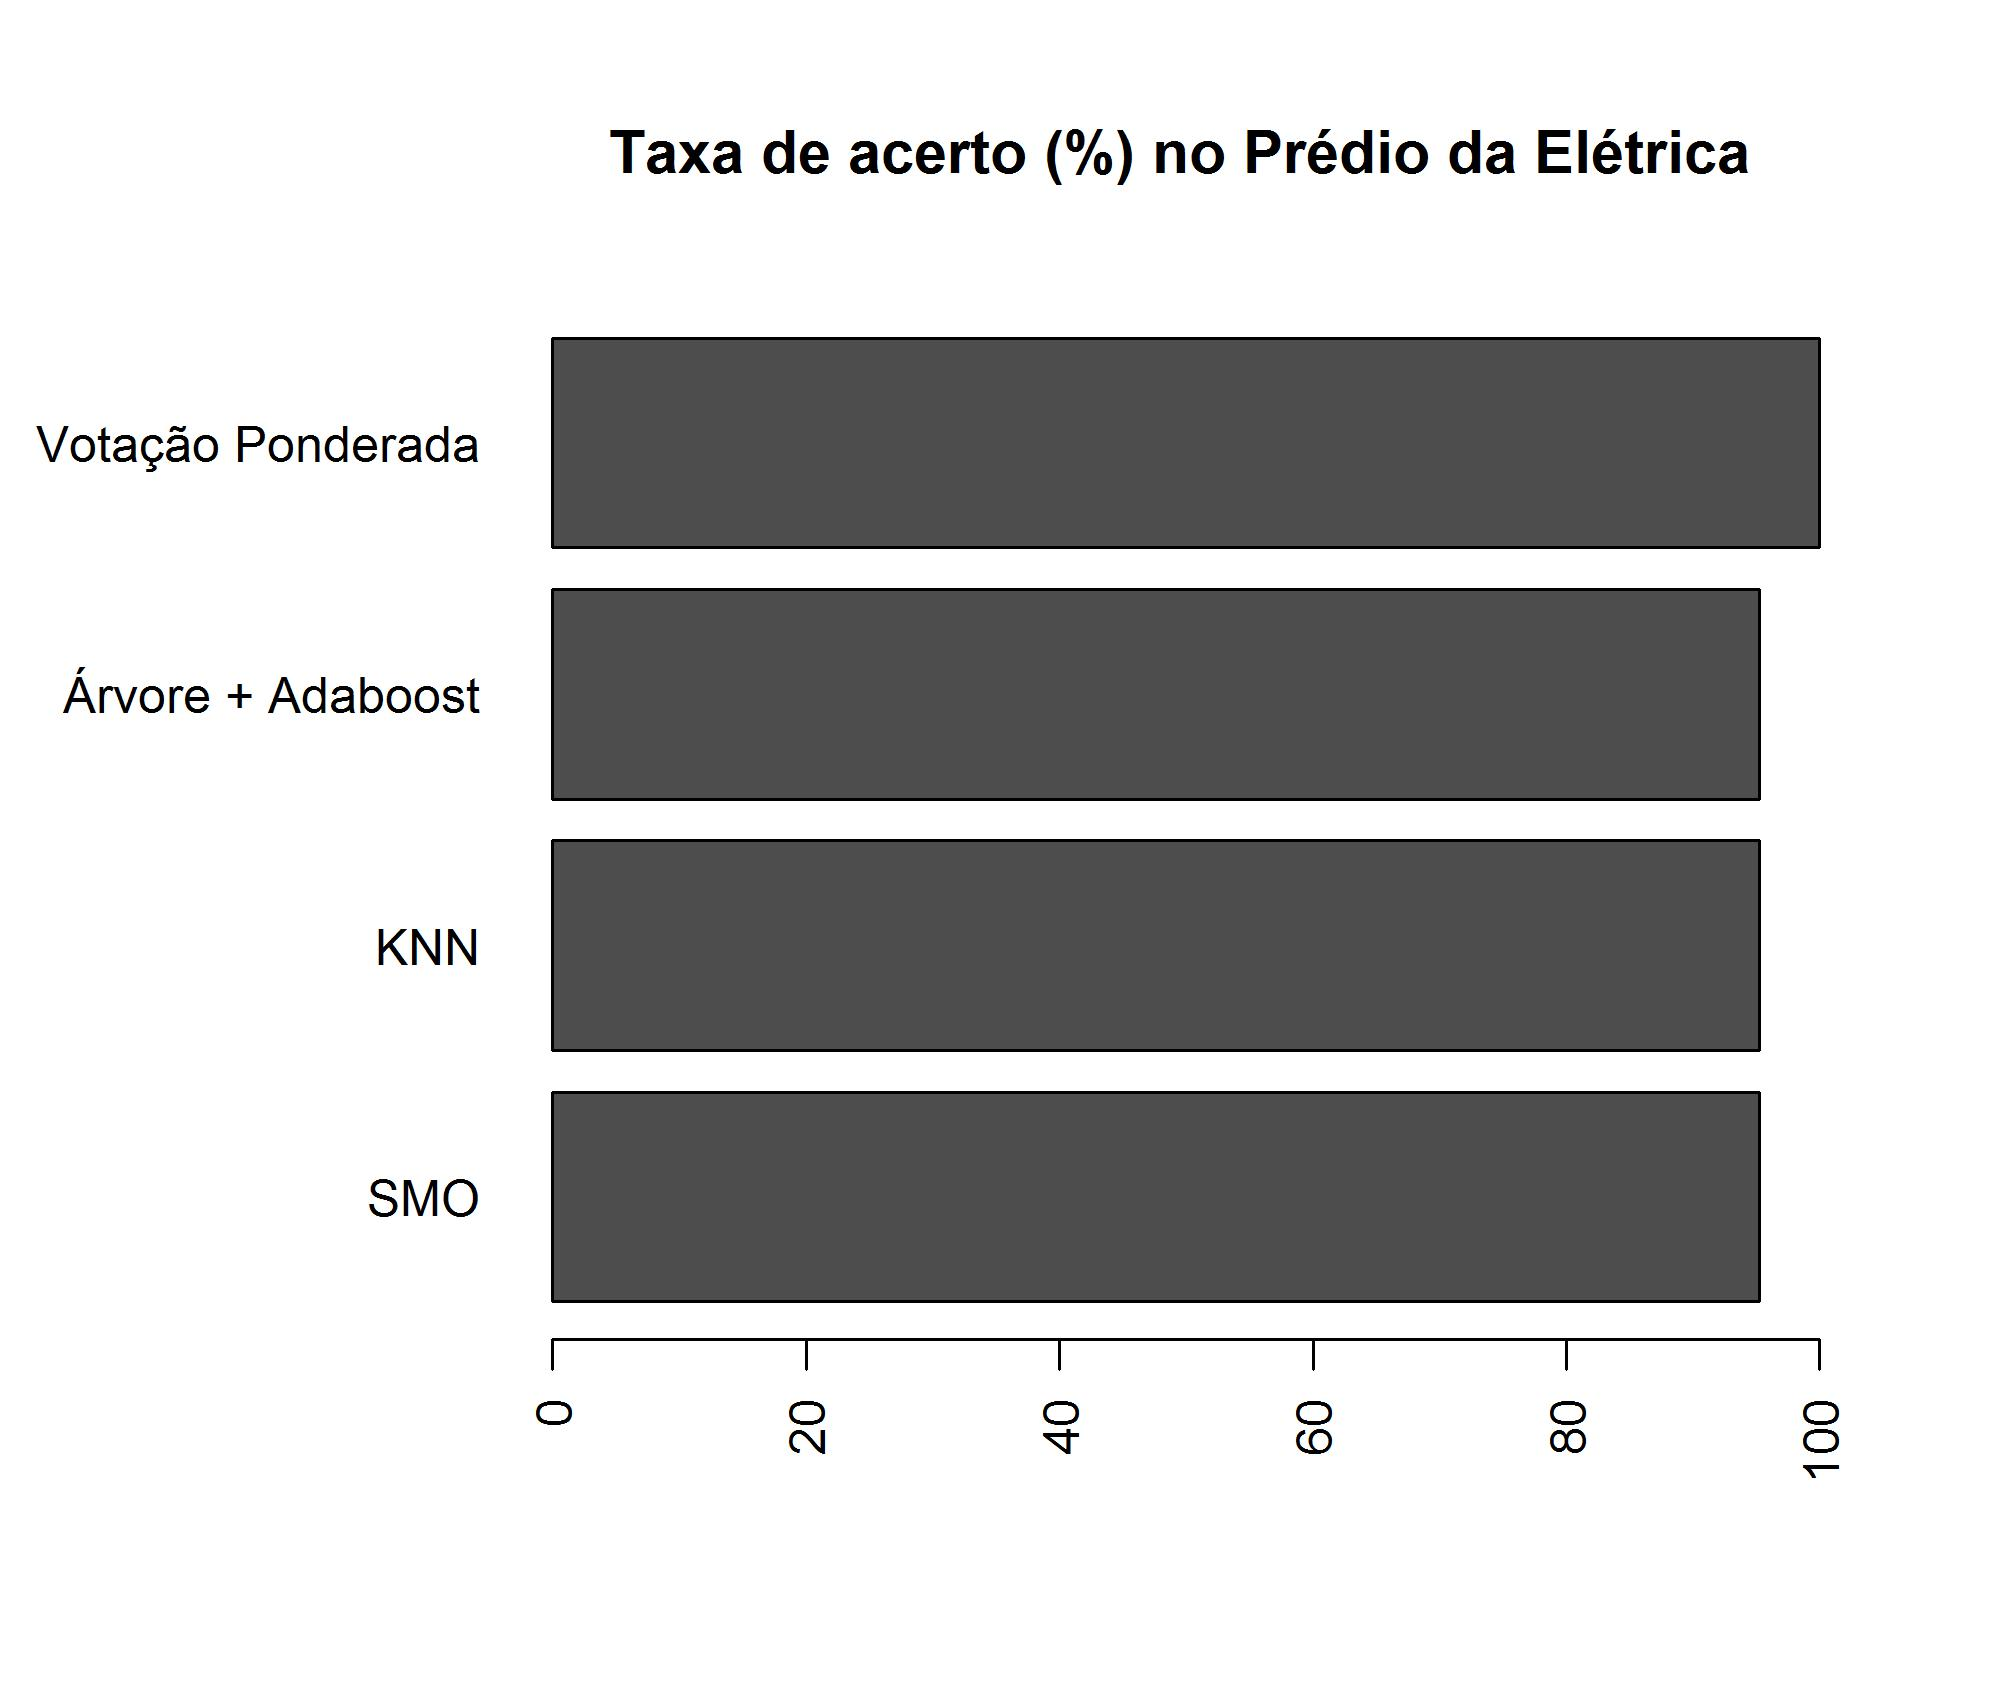
\includegraphics[width=0.7\textwidth]{eletrica_media}
\label{fig:eletricaMedia}

\end{figure}


\begin{figure}[H]

\centering
\caption{Acerto de Classificação usando-se o Filtro de Kalmann como método de normalização dos dados}
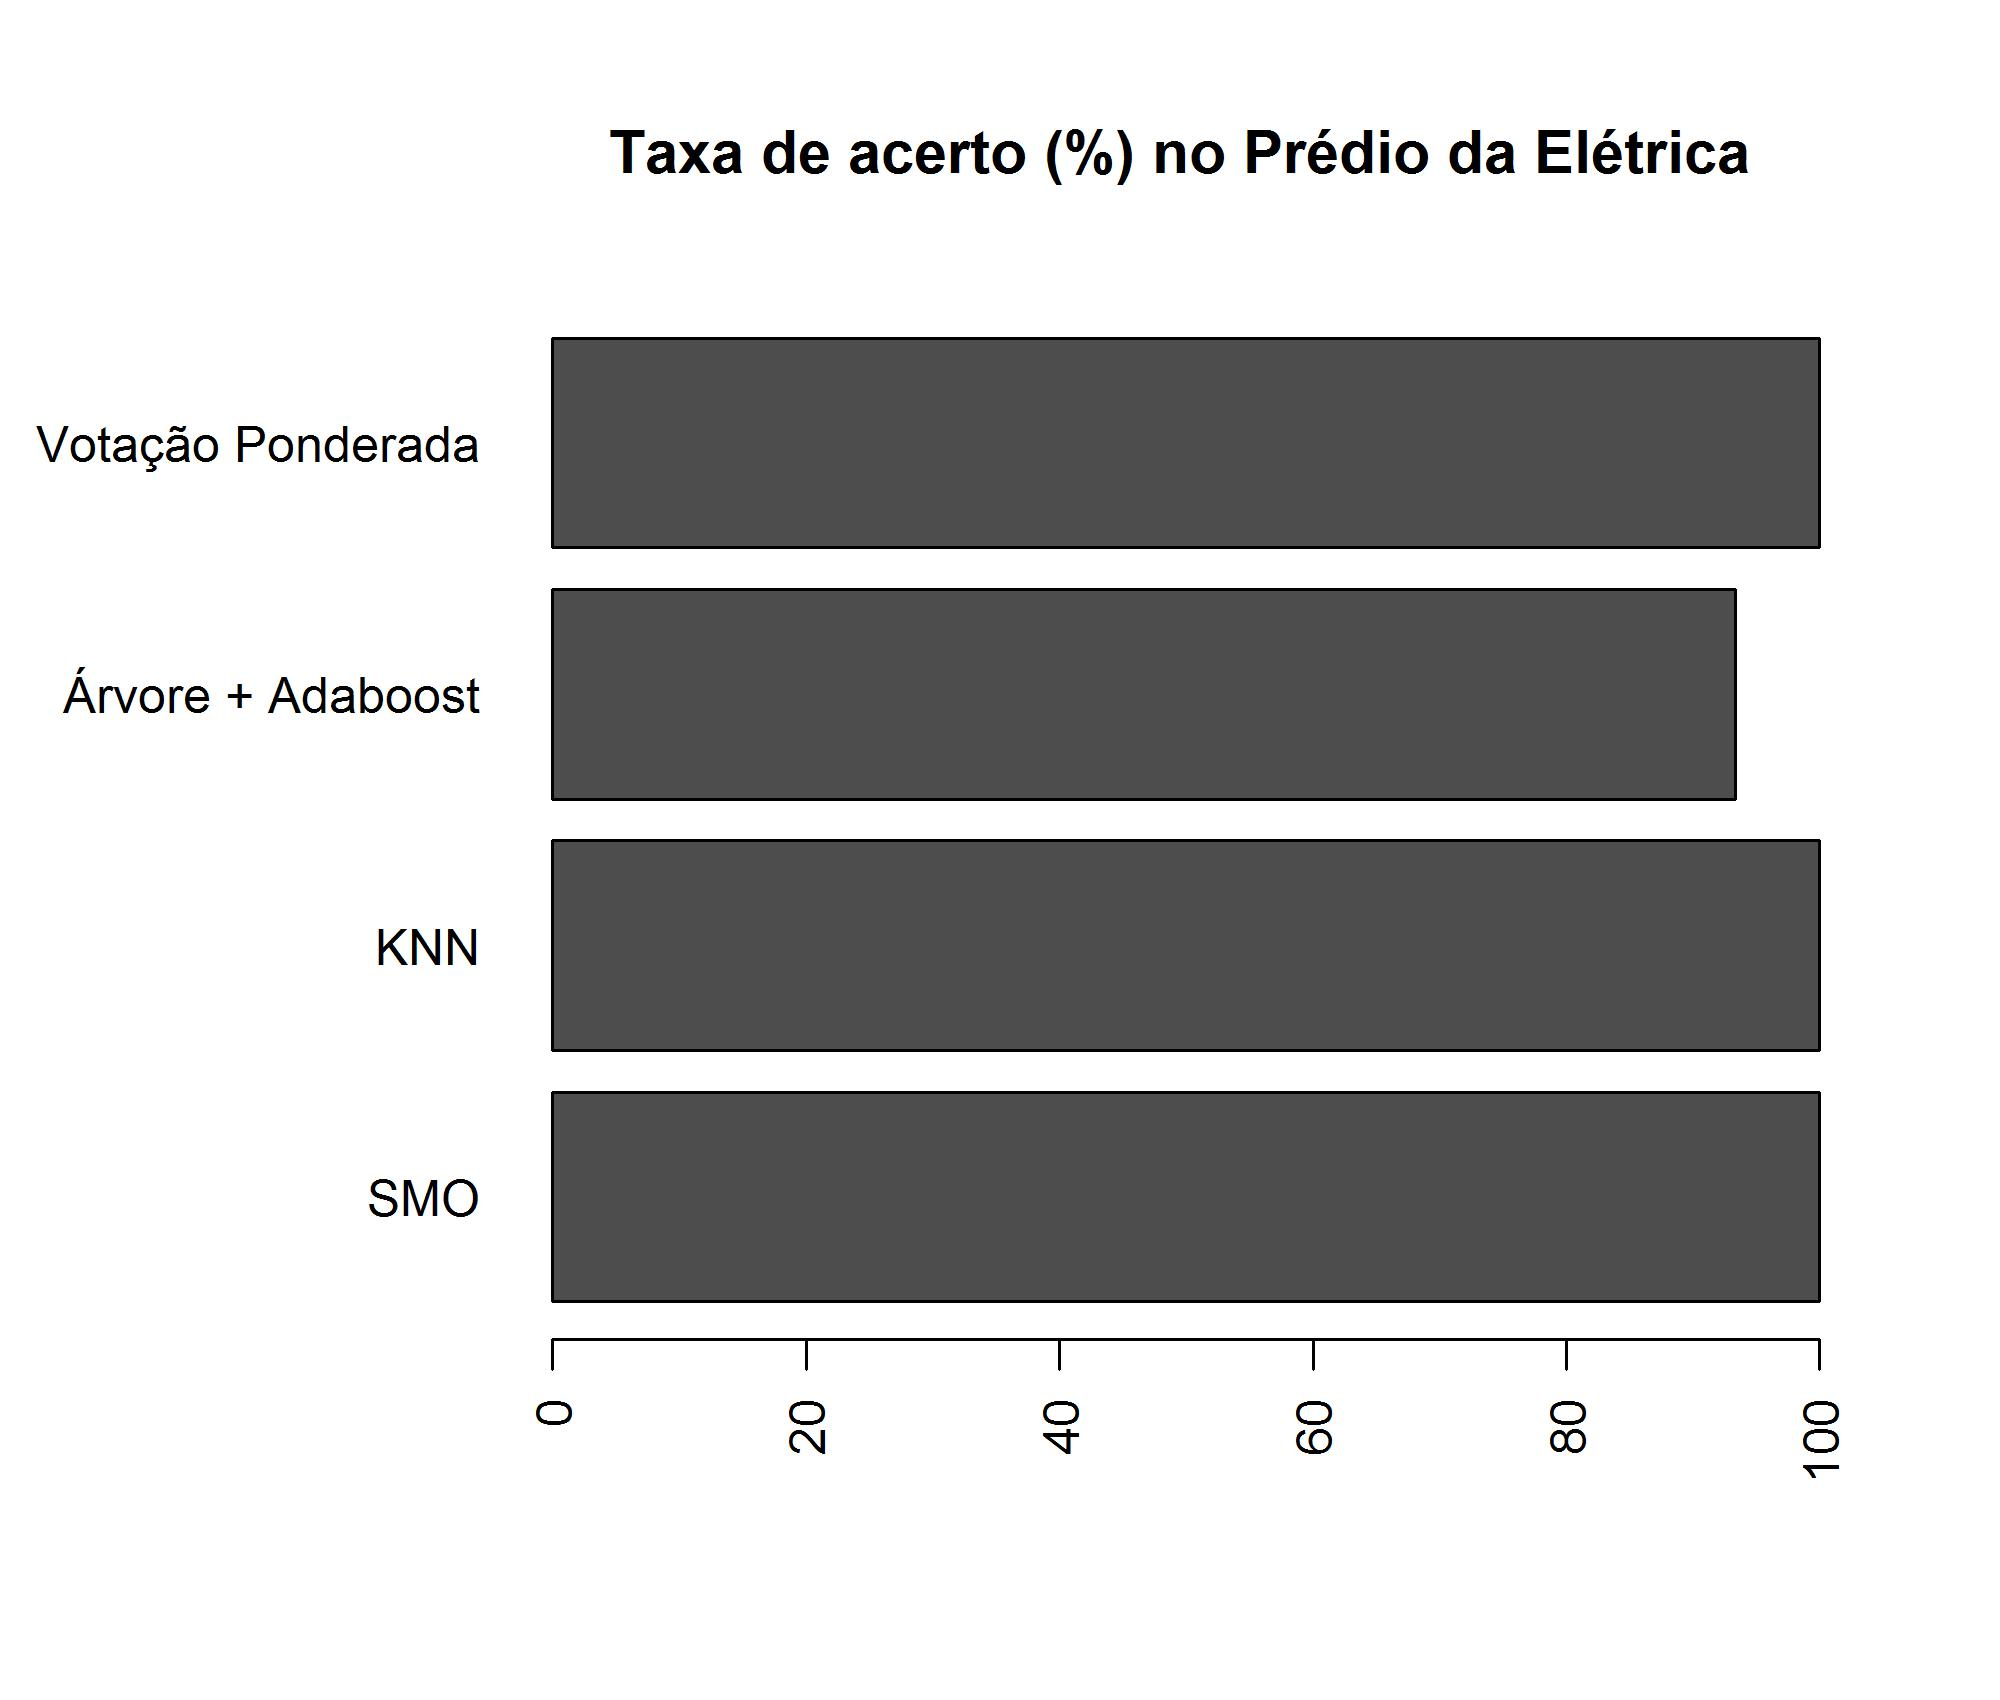
\includegraphics[width=0.7\textwidth]{eletrica_kalman}
\label{fig:eletricaKalman}

\end{figure}

Como é possível observar, tanto o uso da média aritmética quanto o filtro de Kalman como método de normalização acabaram apresentando acerto máximo (100\%) nos testes dentro da Poli-Elétrica.


\section{Objetivos e Resultados}
Tendo em vista o principal objetivo proposto para o projeto, que era desenvolver um conjunto de recursos que possibilitasse o mapeamento e identificação de áreas dentro de ambiente fechados, podemos dizer que o sistema desenvolvido conseguiu alcançá-lo parcialmente.\par
Nas fases iniciais do projeto, as primeiras concepções desenhadas previam a criação de um sistema muito semelhante ao GPS, só que para ambientes fechados. Ou seja, havia a ideia de que o sistema seria capaz de determinar a posição do usuário com a precisão de metros dentro de uma sala. Por exemplo, o sistema seria capaz de determinar se ele está mais perto da janela ou da porta da sala.\par
Porém, como foi constatado posteriormente durante a implementação do projeto, notou-se que existia um \textit{trade-off} claro: Poderíamos abandonar a ideia de localizar o usuário com a precisão geométrica, para localiza-lo com mais precisão a respeito da zona que ele se encontra no prédio. E nesse escopo foram obtidos resultados bastante razoáveis.\par
Além do objetivo principal, durante o desenvolvimento do trabalho surgiu o objetivo da demonstração de uma prova de conceito, para o qual foram desenvolvidos os aplicativos \textit{APScanner} e o \textit{EletricaGO}. Os resultados obtidos a partir destes aplicativos foram usados para demonstrar o funcionamento das ferramentas desenvolvidas e uma das aplicações possíveis para o futuro.\par
O \textit{APScanner} é importante para ilustrar o processo de aquisição dos sinais e seu envio para o servidor, com o posterior treinamento e a possibilidade imediata de testar o mapeamento feito. Por sua vez, o \textit{EleticaGO} serve para apresentar uma aplicação contextual para o sistema, que usa as ferramentas desenvolvidas por meio da nossa API. \par



